\documentclass[conference]{IEEEtran}
\IEEEoverridecommandlockouts
% The preceding line is only needed to identify funding in the first footnote. If that is unneeded, please comment it out.
%Template version as of 6/27/2024
\newcommand{\etal}{\textit{et al.}}
\usepackage{cite}
\usepackage{amsmath,amssymb,amsfonts}
\usepackage{algorithmic}
\usepackage{graphicx}
\usepackage{textcomp}
\usepackage[most]{tcolorbox}
\usepackage{xcolor}
\usepackage{url}
\usepackage{balance}
\usepackage[most]{tcolorbox}
\usepackage{caption}
\usepackage{multirow}


% \def\BibTeX{{\rm B\kern-.05em{\sc i\kern-.025em b}\kern-.08em
%     T\kern-.1667em\lower.7ex\hbox{E}\kern-.125emX}}
\begin{document}

\title{Replicating and Extending SIDE for Code Summary Evaluation and Data Filtering\\}

\author{\IEEEauthorblockN{Zaiyu Cheng}
\IEEEauthorblockA{\textit{Department of Computer Science} \\
\textit{The College of William and Mary}\\
Williamsburg, VA \\
zcheng06@wm.edu}
% \and
% \IEEEauthorblockN{2\textsuperscript{nd} Given Name Surname}
% \IEEEauthorblockA{\textit{dept. name of organization (of Aff.)} \\
% \textit{name of organization (of Aff.)}\\
% City, Country \\
% email address or ORCID}
}
\maketitle

\begin{abstract}
Modern code summarization systems are commonly evaluated with reference-based metrics that measure lexical or surface-level similarity between a generated summary and a reference comment. This assumption is fragile: repository comments may be incomplete or outdated, while a generated summary can describe the code correctly using different wording. This paper studies SIDE, a semantic metric that scores the alignment between a code fragment and a natural-language summary directly. The work has two parts. First, we replicate the original Java study by recovering the experimental artifact, rebuilding the required environment and data dependencies, and rerunning the human-judgment analysis. The reproduced analysis preserves the central claim of the original work: higher SIDE scores are positively associated with better human ratings across overall quality, content adequacy, conciseness, and fluency. Second, we extend the idea to Python by training a Python-specific SIDE metric with code, good-summary, and bad-summary triplets; using it to filter a Python code-summary training set; and comparing a summarization model trained on filtered data with a size-matched unfiltered control. The extension improves average evaluation scores and the monotonic relationship between SIDE and other quality measures, while reducing unstable generation behavior, including very short and empty summaries. These results position SIDE as both a code-summary evaluation metric and a filtering signal for constructing higher-alignment summarization training data. The framework is available at GitHub\footnote{\url{https://github.com/ChrisCheng816/SidePython}}.
\end{abstract}

\begin{IEEEkeywords}
Artificial Intelligence for Software Engineering, CodeT5, Code Summarization
\end{IEEEkeywords}

\section{Introduction}

Automatic code summarization aims to generate short natural-language descriptions of program behavior~\cite{haiduc2010use,sridhara2010towards,mcburney2014automatic,allamanis2016convolutional,iyer2016summarizing,leclair2019neural}. These summaries can support code search, program comprehension, documentation maintenance, and onboarding~\cite{husain2019codesearchnet,lu2021codexglue}. Because manually evaluating generated summaries is expensive, most empirical work relies on automatic metrics that compare a generated summary with a reference comment~\cite{roy2021reassessing,shi2022evaluation,mastropaolo2024evaluating}. Such metrics are convenient and reproducible, but they encode a narrow assumption: a good generated summary should look like the available reference~\cite{papineni2002bleu,lin2004rouge,banerjee2005meteor,popovic2015chrf,zhang2019bertscore}.

That assumption is often weak in software repositories. Reference comments may be stale, incomplete, overly generic, or only loosely connected to the current implementation~\cite{roy2021reassessing,shi2022evaluation,mastropaolo2024evaluating}. At the same time, two summaries can use different wording while expressing the same behavior~\cite{zhang2019bertscore,ren2020codebleu,eghbali2022crystalbleu}. A metric based mainly on token overlap may therefore penalize a faithful generated summary simply because it is phrased differently from the reference~\cite{papineni2002bleu,lin2004rouge,banerjee2005meteor}. This problem motivates evaluation methods that consider the relationship between the code and the summary directly, rather than treating the reference comment as the only source of truth~\cite{mastropaolo2024evaluating}.

The SIDE metric addresses this issue by measuring semantic alignment between code and natural language~\cite{mastropaolo2024evaluating}. Instead of only comparing a generated summary to a reference, SIDE represents code and summaries in a shared embedding space and assigns higher scores when a summary is closer to the code it describes. The original Java study trained this representation with contrastive triplets consisting of code, a suitable summary, and an unsuitable summary, following the general principle of triplet-loss representation learning~\cite{schroff2015facenet,song2020mpnet}. It then evaluated whether the resulting metric was associated with human judgments of summary quality. The key scientific claim is that code-aware semantic alignment provides information that is not fully captured by lexical overlap metrics~\cite{roy2021reassessing,shi2022evaluation,mastropaolo2024evaluating}.

This report first performs a replication of the Java study. The goal of the replication is not to redesign the metric, but to determine whether the original artifact can be recovered and whether the main empirical conclusion still holds when the analysis is rerun locally. After restoring the required data, model assets, execution environment, and statistical workflow, we rerun the human-judgment analysis on the valid annotated examples used for the regression study. The replicated results are reported as odds ratios so they can be compared directly with the original paper.

The second part extends SIDE to Python. We train a Python-specific version of the metric using triplets composed of code, a semantically aligned summary, and a mismatched summary. We then use the trained metric to filter a Python code-summary training set with a high semantic-alignment threshold. The filtered subset retains 17,137 training instances, which is about 6.85\% of the training data. To isolate the effect of semantic filtering from the effect of training-set size, we also create an unfiltered control group with the same number of examples. A CodeT5+(770M) model is trained separately under the unfiltered and SIDE-filtered conditions, then evaluated on generated summaries using standard automatic metrics and an LLM-based judge (GPT-5.3) with scores from 1 to 5~\cite{feng2020codebert,guo2020graphcodebert,guo2021unixcoder,wang2021codet5,wang2023codet5,liu2023geval,zheng2023judging,wang2024large}.

This design turns SIDE from only an evaluation metric into a data-centric filtering signal. If SIDE filtering merely removes data without improving training quality, the filtered model should not consistently outperform the size-matched control. If the metric identifies higher-quality code-summary pairs, however, the filtered condition should produce better summaries and show stronger agreement between SIDE and other quality indicators. The extension results support the latter interpretation: SIDE filtering improves average scores, strengthens the monotonic relationship between SIDE and other metrics, and reduces short or empty generations.

The paper makes three contributions: 

\begin{itemize}
    \item It documents a replication of the original Java SIDE analysis and provides reproduced odds-ratio results for comparison with the original study.
    \item It adapts the SIDE training and scoring workflow to Python code summarization.
    \item It evaluates SIDE-based filtering as a training-data selection strategy, showing that semantic filtering can improve both summary quality and the stability of model outputs.
\end{itemize}


\section{Background and Related Work}

Code summarization is usually evaluated against a reference comment. BLEU, ROUGE, and METEOR operationalize this comparison through n-gram overlap or aligned unigrams~\cite{papineni2002bleu,lin2004rouge,banerjee2005meteor}; ChrF and TF--IDF cosine provide character-level and sparse-vector alternatives~\cite{popovic2015chrf,ramos2003using}. These measures are inexpensive and support consistent comparisons across runs. Their limitation is structural rather than incidental: they estimate agreement with one available comment, not whether the summary is faithful to the implementation. In repositories, where comments can be stale, underspecified, or phrased differently from an equally valid generated summary, this distinction matters~\cite{roy2021reassessing,shi2022evaluation,mastropaolo2024evaluating}.

\subsection{Semantic and Code-Aware Evaluation}

Embedding-based metrics soften the dependence on exact wording. BERTScore, for example, compares contextual token representations and can recognize related surface forms~\cite{zhang2019bertscore}. Yet it remains a comparison between generated and reference text. Code-oriented representation models such as CodeBERT, GraphCodeBERT, and CodeT5 show that code and natural language can be embedded or generated jointly~\cite{feng2020codebert,guo2021graphcodebert,wang2021codet5,wang2023codet5plus}. This makes direct code--summary comparison feasible, but it does not by itself establish an evaluation metric.

CodeBLEU and CrystalBLEU make a related point from code-generation evaluation: surface overlap becomes more meaningful when program structure and ubiquitous tokens are treated explicitly~\cite{ren2020codebleu,eghbali2022crystalbleu}. Their target is generated code rather than generated documentation, but the underlying lesson carries over. Evaluation for software artifacts should account for semantic or structural evidence that a text-only reference comparison cannot observe.

SIDE takes this step for code summaries. It learns a joint representation in which a code fragment is close to an appropriate summary and distant from an inappropriate one~\cite{mastropaolo2024evaluating}. The training formulation follows triplet learning~\cite{schroff2015facenet}: code is the anchor, a matched summary is positive, and a mismatched summary is negative. MPNet supplies the sentence-embedding backbone~\cite{song2020mpnet}. Unlike a reference-only score, SIDE can assign a high value to a paraphrase when that paraphrase remains aligned with the implementation. The present study tests whether this property survives replication and whether it is useful for selecting training data.

\subsection{LLM-Based Judging}

LLM judges offer a complementary route to evaluating generated summaries. With an explicit rubric, they can assess faithfulness, conciseness, and fluency without requiring exact lexical agreement~\cite{liu2023geval,zheng2023judging}. They are not a replacement for controlled automatic metrics: their judgments can reflect prompt design, model preferences, and evaluation variance. We therefore use the LLM judge as an additional code-grounded signal alongside reference-based metrics and SIDE, rather than treating it as an oracle.

\section{Preliminaries}

\subsection{MPNet Encoder}

MPNet is a pre-trained language model that combines masked language modeling and permuted language modeling to learn strong contextual representations~\cite{song2020mpnet}. Its design allows it to model bidirectional context while also learning dependency information from permuted token orders, making it effective for sentence-level semantic representation.

In this work, MPNet is used as the encoder backbone for learning code-summary alignment. Given a code fragment and a natural-language summary, the encoder maps both inputs into a shared semantic space. The resulting representations allow the metric to compare whether a summary is semantically close to the code it describes, rather than only whether it overlaps with a reference summary.

\subsection{CodeT5+ Summarization Model}
CodeT5+ is a family of code-focused encoder-decoder models designed for code understanding and generation tasks~\cite{wang2023codet5plus}. It extends the CodeT5 line of models with flexible encoder-decoder components and pre-training objectives that support tasks such as code generation, code completion, text-to-code retrieval, and code summarization.

In this project, CodeT5+ with 770M parameters serves as the downstream code summarization model. The model is trained under two conditions: one using an unfiltered training set and one using a SIDE-filtered training set. This setup allows the experiment to test whether semantic filtering improves the quality and stability of generated Python summaries.

\subsection{Contrastive Learning}
Contrastive learning trains a representation space by pulling semantically related examples closer together and pushing unrelated examples farther apart. A common form is triplet learning, where each training example contains an anchor, a positive example, and a negative example~\cite{schroff2015facenet}. The model is optimized so that the anchor is closer to the positive example than to the negative example by a margin.

In this work, the anchor is the code fragment, the positive example is a suitable summary, and the negative example is an unsuitable summary. This training objective teaches the metric to distinguish summaries that are semantically aligned with the code from summaries that are not. After training, the learned embedding space is used to score code-summary pairs and to filter training data according to semantic alignment.

\section{Methodology}

The methodology consists of two connected stages. The first stage replicates the original Java-based SIDE study to examine whether the reported association between SIDE and human judgments can be recovered from the released artifact. The second stage adapts SIDE to Python and uses the resulting metric as a filtering signal for code-summary training data.

\begin{figure*}[t]
    \centering
    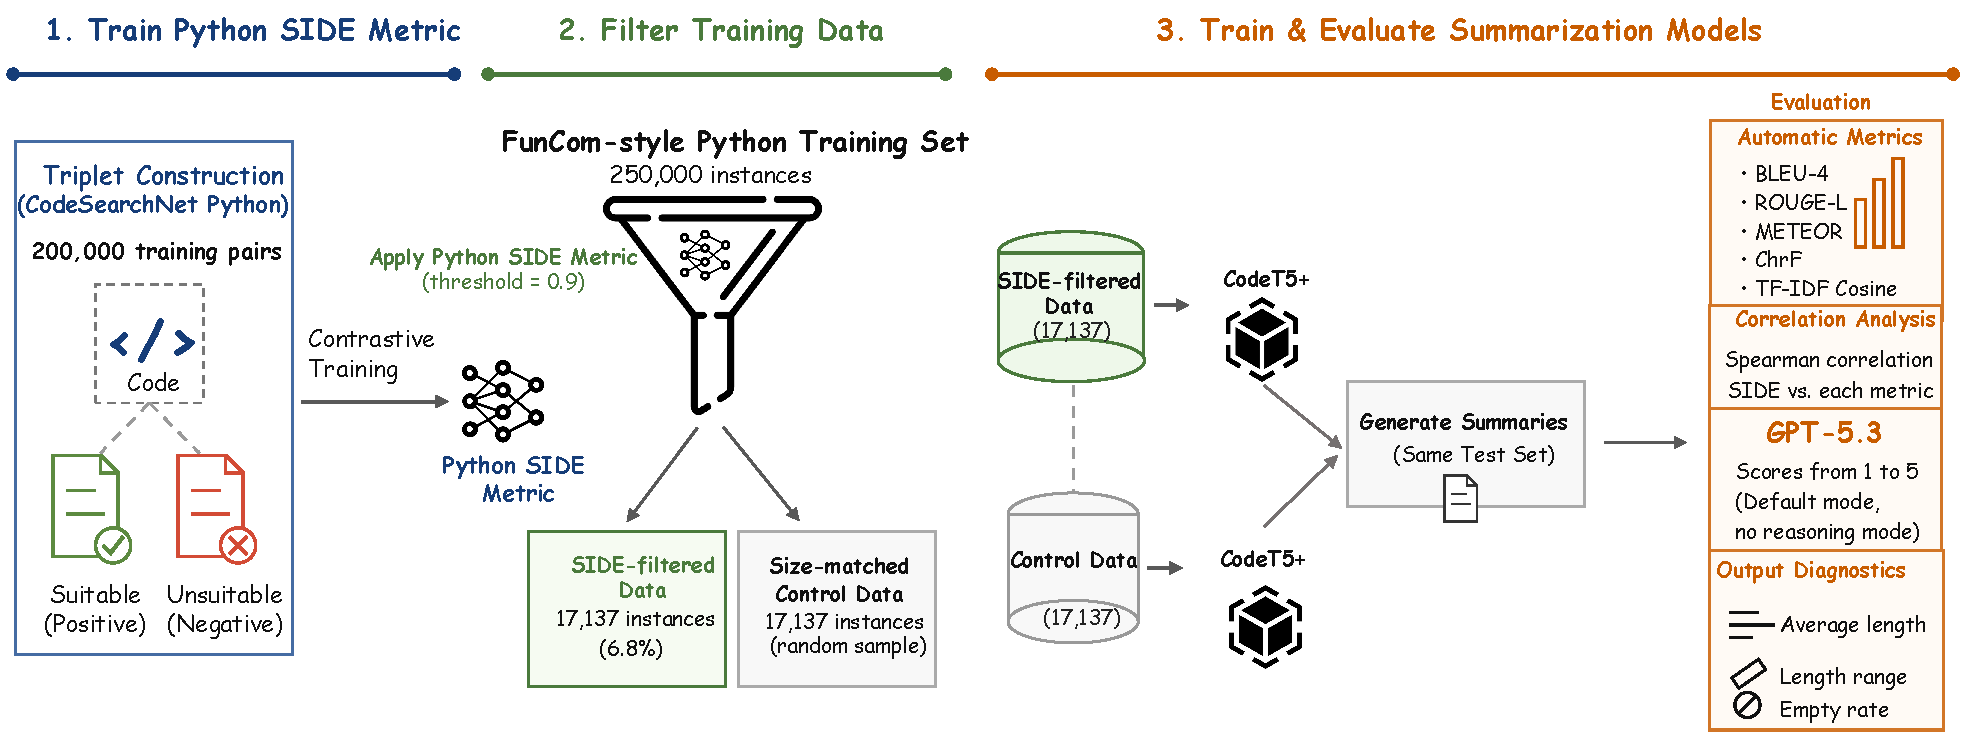
\includegraphics[width=\textwidth]{workflow.pdf}
    \caption{Overview of the Python SIDE extension workflow.}
    \label{fig:python-side-workflow}
\end{figure*}

\subsection{Replication Methodology}

The replication follows the design of the original SIDE paper~\cite{mastropaolo2024evaluating}. The original study frames code summarization evaluation as a code--text alignment problem rather than only as reference-summary matching. In its contrastive formulation, the code fragment serves as the anchor, a suitable summary serves as the positive example, and an unsuitable summary serves as the negative example.

The replication began with artifact recovery. Although the released artifact included the main training, scoring, and statistical-analysis scripts, it was not directly executable in a clean local environment. Some required resources were distributed outside the artifact, and several scripts assumed machine-specific paths or environment variables. The execution environment was therefore reconstructed, the missing training and evaluation resources were restored, and the analysis was rerun locally before comparing the reproduced results with the reported ones.

The SIDE training objective was kept unchanged. The model learns a shared embedding space in which code fragments are closer to suitable summaries than to unsuitable ones. Following the original setup, MPNet is used as the encoder and triplet loss as the contrastive objective. Negative summaries are constructed in two forms: randomly sampled summaries from other examples and hard negatives that remain related to the code but omit part of its behavior. This distinction is important because an incorrect generated summary is often not arbitrary; it may describe the code only partially.

The replication uses the same human-judgment benchmark as the original analysis. The benchmark contains developer ratings for automatically generated summaries of Java methods. Developer-written reference summaries are excluded from the regression analysis, since the comparison is intended to evaluate generated summaries rather than references themselves. After this filtering step, the analysis set contains 5,201 annotated code-summary evaluations.

SIDE is evaluated together with the automatic metrics used in the original study, including lexical-overlap, character-level, embedding-based, and code-summary alignment metrics. This comparison examines whether SIDE behaves similarly to reference-based metrics or captures a distinct aspect of summary quality. The original metric-comparison procedure and statistical modeling pipeline are rerun so that the reproduced results can be compared with the reported findings.

The statistical analysis follows two steps. Relationships among automatic metrics are first examined using rank-based correlation and dimensionality reduction, which indicates whether SIDE clusters with reference-based metrics or forms a separate evaluation dimension. Ordered logistic regression is then used to estimate the association between each metric and the human-rated quality dimensions: direct assessment, content adequacy, conciseness, and fluency. The replicated quantities of interest are odds ratios; values above one indicate that higher metric scores are associated with higher odds of receiving a better human rating.

\subsection{Extension Methodology}

Figure~\ref{fig:python-side-workflow} summarizes the Python extension. In this stage, SIDE is adapted from Java to Python and used as a data-centric filtering signal rather than only as an evaluation metric. The workflow consists of training a Python-specific SIDE metric, filtering Python code-summary pairs, and comparing summarization models trained with and without this filtering step.

Python SIDE is trained with contrastive triplets. Each triplet contains a Python code fragment, its matched ground-truth summary, and a randomly sampled mismatched summary. The code fragment is treated as the anchor, the matched summary as the positive example, and the mismatched summary as the negative example. Training encourages aligned code-summary pairs to have higher cosine similarity than mismatched pairs in the shared semantic space.

After training, the Python SIDE model scores the FunCom-style Python training pairs. A threshold of 0.9 is used to retain only pairs whose code and summary are strongly aligned. Because this filtering changes the size of the training set, a size-matched control set is constructed by randomly sampling the same number of examples from the unfiltered data. This yields two training conditions: a SIDE-filtered set and an unfiltered size-matched control set.

Next, the same CodeT5+ summarization model is trained under both conditions. The architecture and training configuration are fixed across runs, so the comparison isolates the effect of training-data filtering rather than model capacity or optimization choices. Both trained models then generate summaries for the same Python benchmark examples.

The generated summaries are evaluated with BLEU-4, ROUGE-L, METEOR, ChrF, TF-IDF cosine similarity, and SIDE. Spearman correlations are computed between SIDE and the remaining metrics to examine whether SIDE filtering changes the monotonic relationship between semantic alignment and existing evaluation signals. As an additional evaluation signal, GPT-5.3 is used in its default mode, without reasoning mode, as an LLM judge that assigns 1--5 quality scores.

Output-level diagnostics are also computed for both conditions, including average generated-summary length, length range, and empty-summary rate. These measurements help distinguish genuine quality differences from degenerate changes in generation behavior, such as producing shorter or empty summaries.
\section{Study Design}

The study is designed as a two-stage empirical workflow. The first stage reproduces the original Java SIDE setting and establishes whether the metric remains associated with human judgments under a local rerun. The second stage adapts the same idea to Python and evaluates whether SIDE can also serve as a data-filtering signal for training a code summarization model. The overall design therefore separates metric replication from metric-driven data selection.

\subsection{Data Sources}

The replication stage uses the Java resources released with the original SIDE study~\cite{mastropaolo2024evaluating}. Following the original setup, SIDE is trained on CodeSearchNet Java code-summary pairs~\cite{husain2019codesearchnet}, with 100{,}000 training triplets and 10{,}000 validation triplets. The released artifact also provides the trained Java metric and the human-judgment benchmark. Before analysis, we downloaded the dataset, introduced missing dependencies, standardized the environment, and verified that the statistical workflow runs end to end.

The extension stage uses Python code-summary data from CodeSearchNet and the CodeXGLUE code-to-text benchmark~\cite{husain2019codesearchnet,lu2021codexglue,yin2018mining}. For Python SIDE training, we construct contrastive triplets from 200{,}000 Python training pairs. For the downstream filtering experiment, we use the FunCom-style Python split~\cite{leclair2019recommendations,leclair2019neural}, with 250{,}000 training, 10{,}000 validation, and 10{,}000 test instances. Table~\ref{tab:data_filtering_audit} reports the data audit and SIDE filtering result. Since no malformed or empty records were found, the reduction comes from semantic filtering rather than data repair.

\begin{table}[t]
\centering
\caption{Data audit and SIDE filtering statistics for the Python extension.}
\label{tab:data_filtering_audit}
\small
\begin{tabular}{lrrrr}
\hline
\textbf{Split} & \textbf{Original} & \textbf{Retained} & \textbf{Rejected} & \textbf{Rate} \\
\hline
Training & 250,000 & 17,137 & 232,863 & 6.85\% \\
Validation & 10,000 & 575 & 9,425 & 5.75\% \\
\hline
Total & 260,000 & 17,712 & 242,288 & 6.81\% \\
\hline
\end{tabular}
\end{table}

The filtering threshold is 0.9. In the training split, SIDE retains 17,137 out of 250,000 examples, leaving 6.85\% of the original training data. Across the two splits, 17,712 out of 260,000 examples are retained, corresponding to an overall retention rate of 6.81\%. We then sample the same number of unfiltered examples as a size-matched control group, so the comparison isolates semantic filtering from training-set size. The same audit and filtering procedure is applied to the validation split; the final evaluation uses a separate human-annotated test set of 500 examples.

\subsection{SIDE-Based Filtering and Control Construction}

Filtering changes both data quality and data quantity. To avoid attributing improvements merely to a smaller training set, we construct a size-matched control condition. The control data is sampled from the unfiltered FunCom Python training set using a fixed random seed 42, and it contains the same number of examples as the SIDE-filtered set. This creates two comparable training conditions:

\[
D_{\text{control}} \subset D_{\text{raw}},
\qquad
|D_{\text{control}}| = |D_{\text{SIDE}}|.
\]

The comparison therefore isolates the effect of semantic filtering while holding training-set size constant.


\subsection{SIDE Metric Training}

SIDE is trained as a contrastive semantic alignment metric. Each training example is constructed as a triplet consisting of a code fragment, its matched ground-truth summary, and a randomly selected mismatched summary. The code fragment serves as the anchor, the corresponding ground-truth summary is treated as the positive example, and the randomly sampled summary is used as the negative example. Through this contrastive objective, the model learns an embedding space in which semantically aligned code-summary pairs are pulled closer together, while mismatched code-summary pairs are pushed farther apart.

For a code fragment \(c\), positive summary \(s^{+}\), and negative summary \(s^{-}\), the triplet loss is:

\[
\mathcal{L}_{\text{SIDE}}
=
\max\left(
d(f(c), f(s^{+}))
-
d(f(c), f(s^{-}))
+
m,
0
\right),
\]

where \(f(\cdot)\) is the encoder, \(d(\cdot,\cdot)\) is the embedding distance, and \(m\) is the margin. The loss encourages the distance between the code and the positive summary to be smaller than the distance between the code and the negative summary.

The Java part follows the original SIDE setup and uses the recovered Java resources to reproduce the metric scoring and human-judgment analysis. The Python part trains a new SIDE model for Python code-summary pairs. The Python metric uses the same triplet-learning principle, but the triplets are constructed from Python functions and Python documentation while the negative summary samples within these triplets are drawn from other code-summary pairs.

After training, the SIDE score for a code-summary pair is computed as cosine similarity in the learned embedding space:

\[
\operatorname{SIDE}(c,s)
=
\frac{f(c) \cdot f(s)}
{\|f(c)\| \|f(s)\|}.
\]

A higher score indicates stronger semantic alignment between the code and the summary.

\subsection{CodeT5+ Training Design}

CodeT5+ is used as the downstream summarization model. We train the same model architecture under two conditions: one model is trained on the size-matched unfiltered control data, and the other is trained on the SIDE-filtered data. The training, validation, and inference settings are kept consistent across both conditions.

The model is trained with the standard sequence-to-sequence objective. Given code \(c\) and target summary tokens \(y_1,\ldots,y_T\), the training loss is:

\[
\mathcal{L}_{\text{sum}}
=
-\sum_{t=1}^{T}
\log p(y_t \mid y_{<t}, c).
\]

This objective teaches the model to generate the reference summary token by token from the input code. During validation, the model with the lowest validation loss is selected. Early stopping is used to prevent overfitting when validation performance stops improving.

\subsection{Inference and Metric Evaluation}

After training, both CodeT5+ models generate summaries for the same human-annotated 500 test samples. The generated summaries are evaluated with BLEU-4, ROUGE-L, METEOR, ChrF, and TF-IDF cosine similarity. These metrics compare generated summaries with reference summaries from different lexical, character-level, and vector-space perspectives.

In addition to average scores, we compute the relationship between SIDE and the other metrics using Spearman rank correlation:

\[
\rho =
\operatorname{corr}
\left(
\operatorname{rank}(x),
\operatorname{rank}(y)
\right).
\]

This is important because the extension does not only ask whether filtering increases average scores. It also asks whether SIDE-filtered training makes semantic alignment more consistently reflected in other evaluation signals.

\subsection{LLM-as-a-Judge Prompt Design}

To complement the automatic metrics, we use an LLM judge to evaluate whether each generated Python summary is faithful, concise, and fluent. The judge receives only the Python code and the generated summary. It is explicitly instructed not to compare the generated summary against a reference summary, because the goal is to evaluate code-summary alignment directly rather than reference overlap.

Figure~\ref{fig:llm_judge_prompt_full} shows the structured prompt used for this evaluation. The system message defines the judge as an expert evaluator for Python code summarization and requires valid JSON output. The user message provides a rubric for three dimensions: content adequacy, conciseness, and fluency. Each dimension is scored from 1 to 5. The final judge score is computed as the average of the three component scores:

\[
S_{\text{LLM}}
=
\frac{
S_{\text{content}}
+
S_{\text{conciseness}}
+
S_{\text{fluency}}
}{3}.
\]

This design makes the LLM evaluation reproducible and parseable. It also separates different quality dimensions: content adequacy captures faithfulness to the code, conciseness captures unnecessary verbosity, and fluency captures grammar and readability.


\begin{center}
\begin{tcolorbox}[
    breakable,
    colback=white,
    colframe=black,
    title=LLM-as-a-Judge Prompt Structure,
    fonttitle=\bfseries
]
\textbf{System Prompt:} \\
\quad "You are an expert evaluator for Python code summarization.\\[1mm]
\quad Your task is to judge a generated natural-language summary for the given Python code.\\[1mm]
\quad Score Content Adequacy, Conciseness, and Fluency separately on a 1--5 scale.\\[1mm]
\quad Return only valid JSON."\\[1mm]

\hfill\tcbox[colframe = black, colback = white, colupper = black, fontupper=\large, nobeforeafter, left=1mm, right=1mm, top=0.5mm, bottom=0.5mm]{System}

\textbf{Instruction:} \\
\quad "Evaluate the generated summary for the Python code below.\\[1mm]
\quad Score each dimension from 1 to 5.\\[1mm]

\quad \textbf{Content Adequacy:}\\
\quad 1: Incorrect or mostly unrelated to the code.\\
\quad 2: Mentions a small part of the code but misses the main behavior or includes major errors.\\
\quad 3: Partially correct, but incomplete, vague, or contains some misleading details.\\
\quad 4: Mostly correct and useful, with only minor omissions or imprecision.\\
\quad 5: Accurate, faithful, and useful. It captures the main purpose and behavior without needing every minor detail.\\[1mm]

\quad \textbf{Conciseness:}\\
\quad 1: Very verbose, redundant, or filled with irrelevant details.\\
\quad 2: Overly long or includes several unnecessary details.\\
\quad 3: Acceptable length but could be more focused.\\
\quad 4: Mostly concise with only minor extra wording.\\
\quad 5: Clear and compact with no unnecessary detail.\\[1mm]

\quad \textbf{Fluency:}\\
\quad 1: Hard to understand due to grammar, wording, or structure.\\
\quad 2: Understandable only with effort; awkward or error-prone wording.\\
\quad 3: Mostly understandable, but with noticeable grammar or phrasing issues.\\
\quad 4: Clear and natural with only minor wording issues.\\
\quad 5: Fluent, grammatical, and easy to read.\\[1mm]

% \quad Important constraints: judge only the generated summary against the code; do not use any reference or ground-truth summary; reward summaries that correctly capture the main purpose and behavior; penalize hallucinated behavior, overly generic summaries, unnecessary verbosity, and readability issues.\\[1mm]

\quad Python code:\\
\quad \{PYTHON CODE\}\\[1mm]

\quad Generated summary:\\
\quad \{GENERATED SUMMARY\}"\\[1mm]

\hfill\tcbox[colframe = black, colback = white, colupper = black, fontupper=\large, nobeforeafter, left=1mm, right=1mm, top=0.5mm, bottom=0.5mm]{User}

\textbf{Answer:} \\
\quad Return exactly this JSON object and nothing else:\\[1mm]
\quad \{\\[1mm]
\quad \quad "content\_adequacy": integer from 1 to 5,\\[1mm]
\quad \quad "conciseness": integer from 1 to 5,\\[1mm]
\quad \quad "fluency": integer from 1 to 5,\\[1mm]
\quad \quad "reason": "one short sentence"\\[1mm]
\quad \}\\[1mm]

\hfill\tcbox[colframe = black, colback = white, colupper = black, fontupper=\large, nobeforeafter, left=1mm, right=1mm, top=0.5mm, bottom=0.5mm]{Assistant}
% \caption{Pseudocode-like representation of the structured LLM-as-a-judge prompt used to evaluate generated Python summaries.}
% \label{fig:llm_judge_prompt}
\end{tcolorbox}
\captionof{figure}{Complete LLM-as-a-judge prompt.}
\label{fig:llm_judge_prompt_full}
\end{center}

\subsection{Robust JSON Recovery for LLM Outputs}

LLM-generated structured outputs may deviate from strict JSON syntax, for example by using single quotes, omitting quotes around keys, leaving trailing commas, or producing incomplete braces. Such formatting errors can cause standard JSON parsing to fail and interrupt the evaluation pipeline. To reduce this failure mode, we adopt \textit{json\_repair}\footnote{\url{https://github.com/mangiucugna/json_repair}}, a lightweight library for repairing invalid JSON-like strings often produced by language models. The repaired string is then passed to the standard JSON parser for downstream processing.

In the evaluation pipeline, each model output is first normalized into a single JSON-like string and then repaired before parsing. After recovery, a strict schema is enforced by extracting only the expected fields: \texttt{content\_adequacy}, \texttt{conciseness}, \texttt{fluency}, and \texttt{reason}. The three score fields must be integers from 1 to 5, while \texttt{reason} is treated as a short textual explanation. If a field is missing or has an invalid type, a safe fallback value is assigned and the case is logged for inspection. This design prevents minor formatting errors from causing sample loss while preserving deterministic evaluation behavior.

\subsection{Output Diagnostics}

Output diagnostics are used to measure generation stability. For each condition, we compute the average summary length, the range of generated summary lengths, and the rate of empty summaries. These diagnostics are important because a model can sometimes achieve nonzero automatic scores while still producing outputs that are too short, empty, or unstable.

The empty-summary rate is computed as:

\[
R_{\text{empty}}
=
\frac{
N_{\text{empty}}
}{
N_{\text{total}}
}
\times 100\%.
\]

\subsection{Training and Inference Configuration}
SIDE-py is trained as a sentence-embedding model initialized from \texttt{microsoft/mpnet-base}. The encoder uses a maximum sequence length of 512 and mean pooling over token representations. Training uses shuffled mini-batches of 16, a maximum of 10 epochs, a 10\% warmup schedule, and early stopping with patience 5. Model selection is based on the validation triplet margin, computed as
\[
\cos(q,p)-\cos(q,n),
\]
where \(q\), \(p\), and \(n\) denote the query, positive, and negative embeddings, respectively.

For CodeT5+ summarization, the source sequence is the tokenized Python code, and the target sequence is the reference docstring. We truncate or pad encoder inputs to 512 tokens and decoder outputs to 128 tokens. Training uses AdamW with learning rate \(2\times10^{-5}\), epsilon \(10^{-8}\), gradient clipping with maximum norm 1.0, and a linear learning-rate schedule with 20\% warmup. The maximum number of epochs is 15, with early stopping patience of 3 based on validation loss. The effective training batch size is 16, implemented with micro-batch size 4 and gradient accumulation over 4 steps.

At inference time, CodeT5+ decoding is deterministic: it uses greedy generation with beam size 1, no sampling, and a maximum output length of 128 tokens. The SIDE-filtered and control models therefore differ only in the training data they receive, while sharing the same model architecture, optimization procedure, and decoding configuration.
\section{Results}
\subsection{Replication Results}

Table~\ref{tab:side_replication_full} compares the original ordered logistic regression results with the reproduced SIDE results. For each human-judgment dimension, we keep the original paper metrics and append a new row, \textit{SIDE (new)}, which reports the reproduced SIDE result from our local replication.

\begin{table*}[t]
\centering
\caption{Original ordered logistic regression results and reproduced SIDE results. The row \textit{SIDE (new)} reports the reproduced result from this replication.}
\label{tab:side_replication_full}
\small
\begin{tabular}{llrrrrr}
\hline
\textbf{Dimension} & \textbf{Metric} & \textbf{OR} & \textbf{Value} & \textbf{Std. Error} & \textbf{$t$-value} & \textbf{$p$-value} \\
\hline

\multirow{11}{*}{Overall DA Score}
& BLEU-1 & 0.9990 & -0.0010 & 0.0017 & -0.5822 & 0.6222 \\
& BERTScore-R & 1.0029 & 0.0029 & 0.0023 & 1.2634 & 0.2943 \\
& SentenceBERT-CS & 1.0057 & 0.0057 & 0.0020 & 2.8882 & 0.0100 \\
& InferSent-CS & 0.9980 & -0.0020 & 0.0025 & -0.8064 & 0.5250 \\
& ROUGE-1-P & 1.0058 & 0.0058 & 0.0018 & 3.2552 & 0.0033 \\
& ROUGE-4-R & 1.0024 & 0.0024 & 0.0011 & 2.1987 & 0.04667 \\
& ROUGE-W-R & 0.9996 & -0.0004 & 0.0017 & -0.2485 & 0.8040 \\
& c\_coeff & 1.0143 & 0.0142 & 0.0012 & 11.4549 & $<0.0001$ \\
& CodeT5-plus-CS & 1.0044 & 0.0044 & 0.0017 & 2.5383 & 0.0220 \\
& SIDE & 1.0205 & 0.0203 & 0.0017 & 11.7029 & $<0.0001$ \\
& \textbf{SIDE (new)} & \textbf{1.0194} & \textbf{0.0192} & \textbf{0.0018} & \textbf{10.8722} & \textbf{$<0.0001$} \\
\hline

\multirow{11}{*}{Content Adequacy}
& BLEU-1 & 0.9672 & -0.0333 & 0.0347 & -0.9615 & 0.4200 \\
& BERTScore-R & 1.0525 & 0.0512 & 0.0468 & 1.0927 & 0.3929 \\
& SentenceBERT-CS & 1.1121 & 0.1063 & 0.0406 & 2.6172 & 0.0225 \\
& InferSent-CS & 1.0000 & 0.0000 & 0.0517 & -0.0004 & 1.0000 \\
& ROUGE-1-P & 1.0943 & 0.0901 & 0.0364 & 2.4733 & 0.0260 \\
& ROUGE-4-R & 0.9914 & -0.0086 & 0.0226 & -0.3814 & 0.7811 \\
& ROUGE-W-R & 1.0437 & 0.0428 & 0.0351 & 1.2202 & 0.3700 \\
& c\_coeff & 1.3729 & 0.3169 & 0.0255 & 12.4350 & $<0.0001$ \\
& CodeT5-plus-CS & 1.1413 & 0.1322 & 0.0358 & 3.6877 & $<0.0001$ \\
& SIDE & 1.6265 & 0.4864 & 0.0366 & 13.2942 & $<0.0001$ \\
& \textbf{SIDE (new)} & \textbf{1.5739} & \textbf{0.4535} & \textbf{0.0373} & \textbf{12.1635} & \textbf{$<0.0001$} \\
\hline

\multirow{11}{*}{Conciseness}
& BLEU-1 & 1.0656 & 0.0636 & 0.0342 & 1.8576 & 0.1575 \\
& BERTScore-R & 1.0160 & 0.0159 & 0.0470 & 0.3375 & 0.8770 \\
& SentenceBERT-CS & 1.0587 & 0.0571 & 0.0403 & 1.4163 & 0.2617 \\
& InferSent-CS & 1.0079 & 0.0079 & 0.0511 & 0.1547 & 0.8770 \\
& ROUGE-1-P & 1.0075 & 0.0075 & 0.0359 & 0.2091 & 0.8770 \\
& ROUGE-4-R & 0.9937 & -0.0063 & 0.0228 & -0.2766 & 0.8770 \\
& ROUGE-W-R & 1.0954 & 0.0911 & 0.0346 & 2.6352 & 0.0267 \\
& c\_coeff & 1.2433 & 0.2178 & 0.0254 & 8.5798 & $<0.0001$ \\
& CodeT5-plus-CS & 1.0630 & 0.0611 & 0.0355 & 1.7212 & 0.1700 \\
& SIDE & 1.3844 & 0.3253 & 0.0354 & 9.1835 & $<0.0001$ \\
& \textbf{SIDE (new)} & \textbf{1.3462} & \textbf{0.2973} & \textbf{0.0361} & \textbf{8.2382} & \textbf{$<0.0001$} \\
\hline

\multirow{11}{*}{Fluency}
& BLEU-1 & 1.0650 & 0.0629 & 0.0345 & 1.8243 & 0.2267 \\
& BERTScore-R & 1.0559 & 0.0544 & 0.0467 & 1.2038 & 0.4600 \\
& SentenceBERT-CS & 0.9958 & -0.0042 & 0.0404 & -0.1043 & 0.9170 \\
& InferSent-CS & 1.0543 & 0.0529 & 0.0515 & 1.0272 & 0.4600 \\
& ROUGE-1-P & 1.0334 & 0.0329 & 0.0365 & 0.9004 & 0.4600 \\
& ROUGE-4-R & 1.0304 & 0.0299 & 0.0229 & 1.3061 & 0.4600 \\
& ROUGE-W-R & 0.9672 & -0.0334 & 0.0347 & -0.9603 & 0.4600 \\
& c\_coeff & 1.2080 & 0.1553 & 0.0253 & 6.1437 & $<0.0001$ \\
& CodeT5-plus-CS & 1.0249 & 0.0246 & 0.0357 & 0.6902 & 0.5444 \\
& SIDE & 1.2826 & 0.2489 & 0.0359 & 6.9359 & $<0.0001$ \\
& \textbf{SIDE (new)} & \textbf{1.2647} & \textbf{0.2348} & \textbf{0.0366} & \textbf{6.4227} & \textbf{$<0.0001$} \\
\hline
\end{tabular}
\end{table*}

The reproduced SIDE results are highly consistent with the original paper. Across all four human-judgment dimensions, \textit{SIDE (new)} remains statistically significant with \(p<0.0001\), and every reproduced odds ratio is greater than 1. This means that higher reproduced SIDE scores are still associated with higher odds of receiving better human ratings.

For Overall DA Score, the reproduced SIDE odds ratio is 1.0194, very close to the original SIDE value of 1.0205. This is one of the strongest pieces of evidence for a successful replication because the overall score is the broadest human quality dimension. The reproduced coefficient is slightly smaller than the original coefficient, but the direction, magnitude, and significance remain almost unchanged.

For Content Adequacy, \textit{SIDE (new)} obtains an odds ratio of 1.5739. This is lower than the original SIDE value of 1.6265, but it is still much larger than the other metrics in the original table. The closest non-SIDE metric is c\_coeff with an odds ratio of 1.3729, followed by CodeT5-plus-CS with 1.1413 and SentenceBERT-CS with 1.1121. This confirms the central role of SIDE: it is especially strong at predicting whether a generated summary contains the right semantic content for the code.

For Conciseness, the reproduced SIDE odds ratio is 1.3462, again slightly below the original SIDE value of 1.3844 but still higher than all other metrics in the original table. The next strongest metric is c\_coeff with an odds ratio of 1.2433, while most lexical and embedding metrics are close to 1 or statistically insignificant. This suggests that SIDE is not only measuring content overlap; summaries that are better aligned with code semantics are also more likely to be judged concise.

For Fluency, \textit{SIDE (new)} has an odds ratio of 1.2647, compared with the original SIDE value of 1.2826. This dimension is less directly tied to code semantics than content adequacy, yet SIDE still outperforms the other metrics in the table. The closest competing metric is c\_coeff with an odds ratio of 1.2080, while CodeT5-plus-CS and most reference-overlap metrics are weaker. This indicates that SIDE captures a quality signal that is broader than lexical similarity alone.

The reproduction preserves the ranking pattern of the original study. SIDE remains the strongest metric among the reported candidates for Content Adequacy, Conciseness, and Fluency, and it remains highly competitive for Overall DA Score. The small decreases from the original SIDE row to \textit{SIDE (new)} are expected in a local artifact rerun because of environment differences, dependency versions, and recovered data assets. However, these differences do not change the interpretation: the reproduced SIDE metric continues to show a robust and statistically significant association with human judgments, especially for semantic content quality.


\subsection{Extension Results}

The Python extension evaluates whether SIDE filtering improves downstream code summarization training. Table~\ref{tab:extension_metrics} compares the unfiltered control condition with the SIDE-filtered condition; Table~\ref{tab:output_diagnostics} reports output-length diagnostics and empty-summary rates. The results are organized around two questions:

\begin{itemize}

    \item Does SIDE filtering improve average evaluation scores and strengthen the correlation between SIDE and other quality signals?

    \item Does SIDE filtering reduce unstable generation behavior, such as empty summaries or abnormal output lengths?
\end{itemize}

\begin{table*}[t]
\centering
\caption{Comparison between unfiltered and SIDE-filtered training conditions. Correlation values are Spearman correlations with SIDE.}
\label{tab:extension_metrics}
\begin{tabular}{lrrrrrr}
\hline
\textbf{Metric} &
\textbf{No Filter Avg.} &
\textbf{SIDE-Filtered Avg.} &
\textbf{$\Delta$ Avg.} &
\textbf{No Filter $\rho$} &
\textbf{SIDE-Filtered $\rho$} &
\textbf{$\Delta \rho$} \\
\hline
BLEU-4 & 5.4121 & 6.3185 & +0.9064 & 0.50 & 0.54 & +0.04 \\
ROUGE-L & 33.4254 & 34.7324 & +1.3070 & 0.55 & 0.60 & +0.05 \\
METEOR & 17.0302 & 18.5237 & +1.4935 & 0.53 & 0.57 & +0.04 \\
ChrF & 24.3055 & 27.4066 & +3.1011 & 0.55 & 0.57 & +0.02 \\
TF-IDF Cosine & 17.1617 & 17.5747 & +0.4130 & 0.52 & 0.59 & +0.07 \\
GPT-5.3 Judge & 2.5080 & 3.1020 & +0.5940 & 0.48 & 0.54 & +0.06 \\
\hline
\end{tabular}
\end{table*}

\paragraph{\textbf{Can filtered training data improve summarization quality?}} Table~\ref{tab:extension_metrics} shows that SIDE filtering improves all average evaluation scores and also strengthens the monotonic relationship between SIDE and the other metrics. This indicates that SIDE filtering has two effects: it improves the generated summaries according to standard evaluation metrics, and it makes SIDE more consistent with the other quality signals.

For lexical overlap, BLEU-4 increases from 5.4121 to 6.3185, a gain of 0.9064 points. This suggests that the SIDE-filtered model produces summaries with more exact phrase-level overlap with the references. Although BLEU-4 is strict and sensitive to wording, the improvement shows that semantic filtering does not hurt surface-level matching; instead, it slightly improves it. The Spearman correlation between BLEU-4 and SIDE also rises from 0.50 to 0.54, meaning that summaries with higher SIDE scores are more consistently ranked higher by BLEU-4 after filtering.

ROUGE-L increases from 33.4254 to 34.7324, a gain of 1.3070 points. Since ROUGE-L measures longest common subsequence overlap, this improvement suggests that SIDE-filtered training helps the model preserve more reference-relevant content in its generated summaries. Its correlation with SIDE also improves from 0.55 to 0.60, which is the strongest post-filtering correlation among the reference-based metrics. This shows that the filtered model produces summaries whose sequence-level overlap is more aligned with semantic code-summary alignment.

METEOR increases from 17.0302 to 18.5237, a gain of 1.4935 points. This is important because METEOR is more tolerant of flexible wording than BLEU and rewards unigram alignment, stemming, and paraphrase-like similarity. The improvement suggests that SIDE filtering helps the model generate summaries that are semantically closer to the reference, even when exact wording differs. The correlation with SIDE also increases from 0.53 to 0.57.

ChrF shows the largest automatic-metric gain, increasing from 24.3055 to 27.4066, a gain of 3.1011 points. Because ChrF is based on character n-gram overlap, this improvement indicates that the SIDE-filtered model produces outputs with stronger fine-grained lexical similarity to the reference. Its correlation with SIDE increases from 0.55 to 0.57, showing a smaller but still positive improvement in metric alignment.

TF-IDF cosine increases from 17.1617 to 17.5747, a smaller gain of 0.4130 points. Although the average improvement is modest, the correlation with SIDE rises from 0.52 to 0.59, which is the largest correlation gain in the table. This suggests that while TF-IDF similarity changes only slightly in average value, its ranking behavior becomes much more consistent with SIDE after filtering.

The GPT-5.3 judge score increases from 2.5080 to 3.1020, a gain of 0.5940 points on a 1--5 scale. This is the additional evidence that the improvement is not limited to automatic reference-based metrics. The LLM judge evaluates whether a summary is faithful and useful for the code, so this increase suggests that SIDE-filtered training improves perceived summary quality. Its correlation with SIDE also rises from 0.48 to 0.54, indicating that the judge becomes more aligned with SIDE under the filtered condition.

We can see every average score increases and every Spearman correlation with SIDE also increases from Table~\ref{tab:extension_metrics}. The average-score gains show that SIDE filtering improves summary quality, while the correlation gains show that the filtered model produces outputs whose quality rankings are more coherent across metrics. This supports the main extension claim that SIDE filtering is not merely removing data; it is selecting training examples that lead to more stable and semantically aligned summarization behavior.


\begin{table}[t]
\centering
\caption{Output length diagnostics for the 500 generated summaries in each condition. Token counts are computed after removing sequence boundary markers.}
\label{tab:output_diagnostics}
\small
\begin{tabular}{lrrr}
\hline
\textbf{Diagnostic} & \textbf{No Filter} & \textbf{SIDE-Filtered} & \textbf{$\Delta$} \\
\hline
Mean length & 7.934 & 9.398 & +1.464 \\
25th percentile & 6 & 6 & 0 \\
Median length & 7 & 8 & +1 \\
75th percentile & 9 & 11 & +2 \\
Minimum length & 0 & 0 & 0 \\
Maximum length & 42 & 34 & -8 \\
Empty summaries & 23 & 6 & -17 \\
Empty summary rate & 4.60\% & 1.20\% & -3.40 pp \\
\hline
\end{tabular}
\end{table}

\paragraph{\textbf{How do the output diagnostics differ after training with different datasets?}} Table~\ref{tab:output_diagnostics} shows that SIDE filtering also improves output stability. The mean generated-summary length increases from 7.934 tokens to 9.398 tokens. More importantly, the distribution shifts upward: the median increases from 7 to 8 tokens, and the 75th percentile increases from 9 to 11 tokens. This suggests that the SIDE-filtered model is not only producing a few longer summaries; its typical output is also more informative.

The lower quartile remains 6 tokens in both conditions, so SIDE filtering does not eliminate short summaries entirely. However, it substantially reduces the most severe failure case: empty outputs. The unfiltered model produces 23 empty summaries out of 500, corresponding to an empty-summary rate of 4.60\%. The SIDE-filtered model produces only 6 empty summaries, reducing the empty-summary rate to 1.20\%. This is a practical improvement because empty summaries are unusable regardless of their metric scores.

The maximum length also decreases from 42 to 34 tokens. Combined with the higher median and higher upper quartile, this suggests that SIDE filtering makes the output distribution more stable: it reduces empty generations while avoiding extremely long outputs. Thus, the output diagnostics support the metric results. SIDE filtering improves several quality measures, increases agreement between SIDE and other metrics, and reduces degenerate generation behavior.


\section{Threats to Validity}

\textbf{Construct validity:} The study uses automatic metrics and an LLM judge as proxies for code summary quality. BLEU-4, ROUGE-L, METEOR, ChrF, and TF-IDF cosine measure different forms of reference similarity, but none of them fully captures whether a summary is useful to a developer. SIDE measures semantic alignment between code and summary, but it is still a learned metric and may prefer summaries that resemble its training distribution. The LLM judge provides an additional quality signal, but its scores may reflect model-specific preferences rather than true human judgment.

\textbf{Internal validity:} The replication results may be affected by artifact recovery decisions, dependency versions, and local execution settings. Although the reproduced SIDE results follow the same statistical workflow as the original study, small differences in restored resources or package behavior can affect coefficient estimates. For the Python extension, performance differences may be influenced by data preprocessing, filtering threshold choice, random sampling of the control group, and training variance. The filtering threshold of 0.9 is interpretable as a high-alignment cutoff, but different thresholds may produce different tradeoffs between data quality and data quantity.

\textbf{Conclusion validity:} The extension reports point estimates for metric scores, correlations, and output diagnostics. The metric improvements are consistent across the reported table, but the magnitude of improvement differs across metrics. In particular, some metrics show larger gains than others, suggesting that SIDE filtering may improve certain aspects of summary quality more strongly than others. The LLM judge result should also be interpreted as supporting evidence rather than definitive proof.

\textbf{External validity:} The replication focuses on the original Java setting, while the extension focuses on Python code summarization. The findings may not generalize to other programming languages, datasets, model families, or documentation styles. The Python extension uses a specific summarization model and a specific SIDE-filtered training setup, so results may differ for larger models, different encoder-decoder architectures, or alternative data selection strategies.

\section{Conclusion}

This paper reproduces and extends SIDE, a semantic metric for code-summary alignment. The replication recovers the Java artifact and reruns the ordered logistic regression analysis on the human-judgment benchmark. The reproduced SIDE results remain statistically significant across overall direct assessment, content adequacy, conciseness, and fluency, preserving the main conclusion of the original study.

The extension adapts SIDE to Python and evaluates it as a data-centric filtering signal. After training a Python-specific SIDE metric, we use it to filter Python code-summary training data and compare a SIDE-filtered training condition against a size-matched unfiltered control. The results show that SIDE filtering improves average scores across BLEU-4, ROUGE-L, METEOR, ChrF, TF-IDF cosine, and the GPT-5.3 judge. It also increases Spearman correlations between SIDE and every other reported metric, suggesting that the filtered model produces summaries whose quality rankings are more consistent across evaluation signals.

Output diagnostics provide additional evidence that SIDE filtering affects generation behavior rather than only metric scores. The filtered model produces fewer empty summaries and a more stable length distribution. These findings suggest that SIDE can be used not only as an evaluation metric, but also as a high-alignment data selection signal for code summarization.
\newpage
\balance
\bibliography{IEEEfull}
\bibliographystyle{IEEEtran}
\end{document}
